\subsection{Диаграмма развертывания приложения}

UML-диаграмма развертывания (англ. deployment diagram) — это графическое представление, которое используется для моделирования физической конфигурации системы и ее компонентов. Она позволяет описать распределение аппаратных и программных ресурсов, а также взаимосвязи между ними.

Диаграмма развертывания помогает визуализировать, как компоненты системы размещаются на аппаратных устройствах (например, серверах, компьютерах, мобильных устройствах), а также как они связаны между собой через сети и каналы связи. Эта диаграмма предоставляет общую картину физического размещения системы и ее взаимодействия с окружающей средой.

% UML-диаграмма развертывания (deployment diagram) является одной из диаграмм в языке моделирования UML,
% которая позволяет визуализировать физическое размещение компонентов программной системы и их взаимосвязи на физических узлах
% (например, серверы, компьютеры или устройства).

% Диаграмма развертывания позволяет показать, какие компоненты программной системы находятся на каких узлах
% и как они взаимодействуют между собой и с внешними ресурсами.
% На диаграмме могут быть отображены узлы (физические или виртуальные),
% компоненты, связи между ними, а также различные артефакты, такие как файлы или базы данных.

Диаграмма развертывания приложения спроектирована в draw.io и представлена на рис.~\ref{fig:UML_deployment_diagram_prod}.

\begin{figure}[!htb]
    \centering

    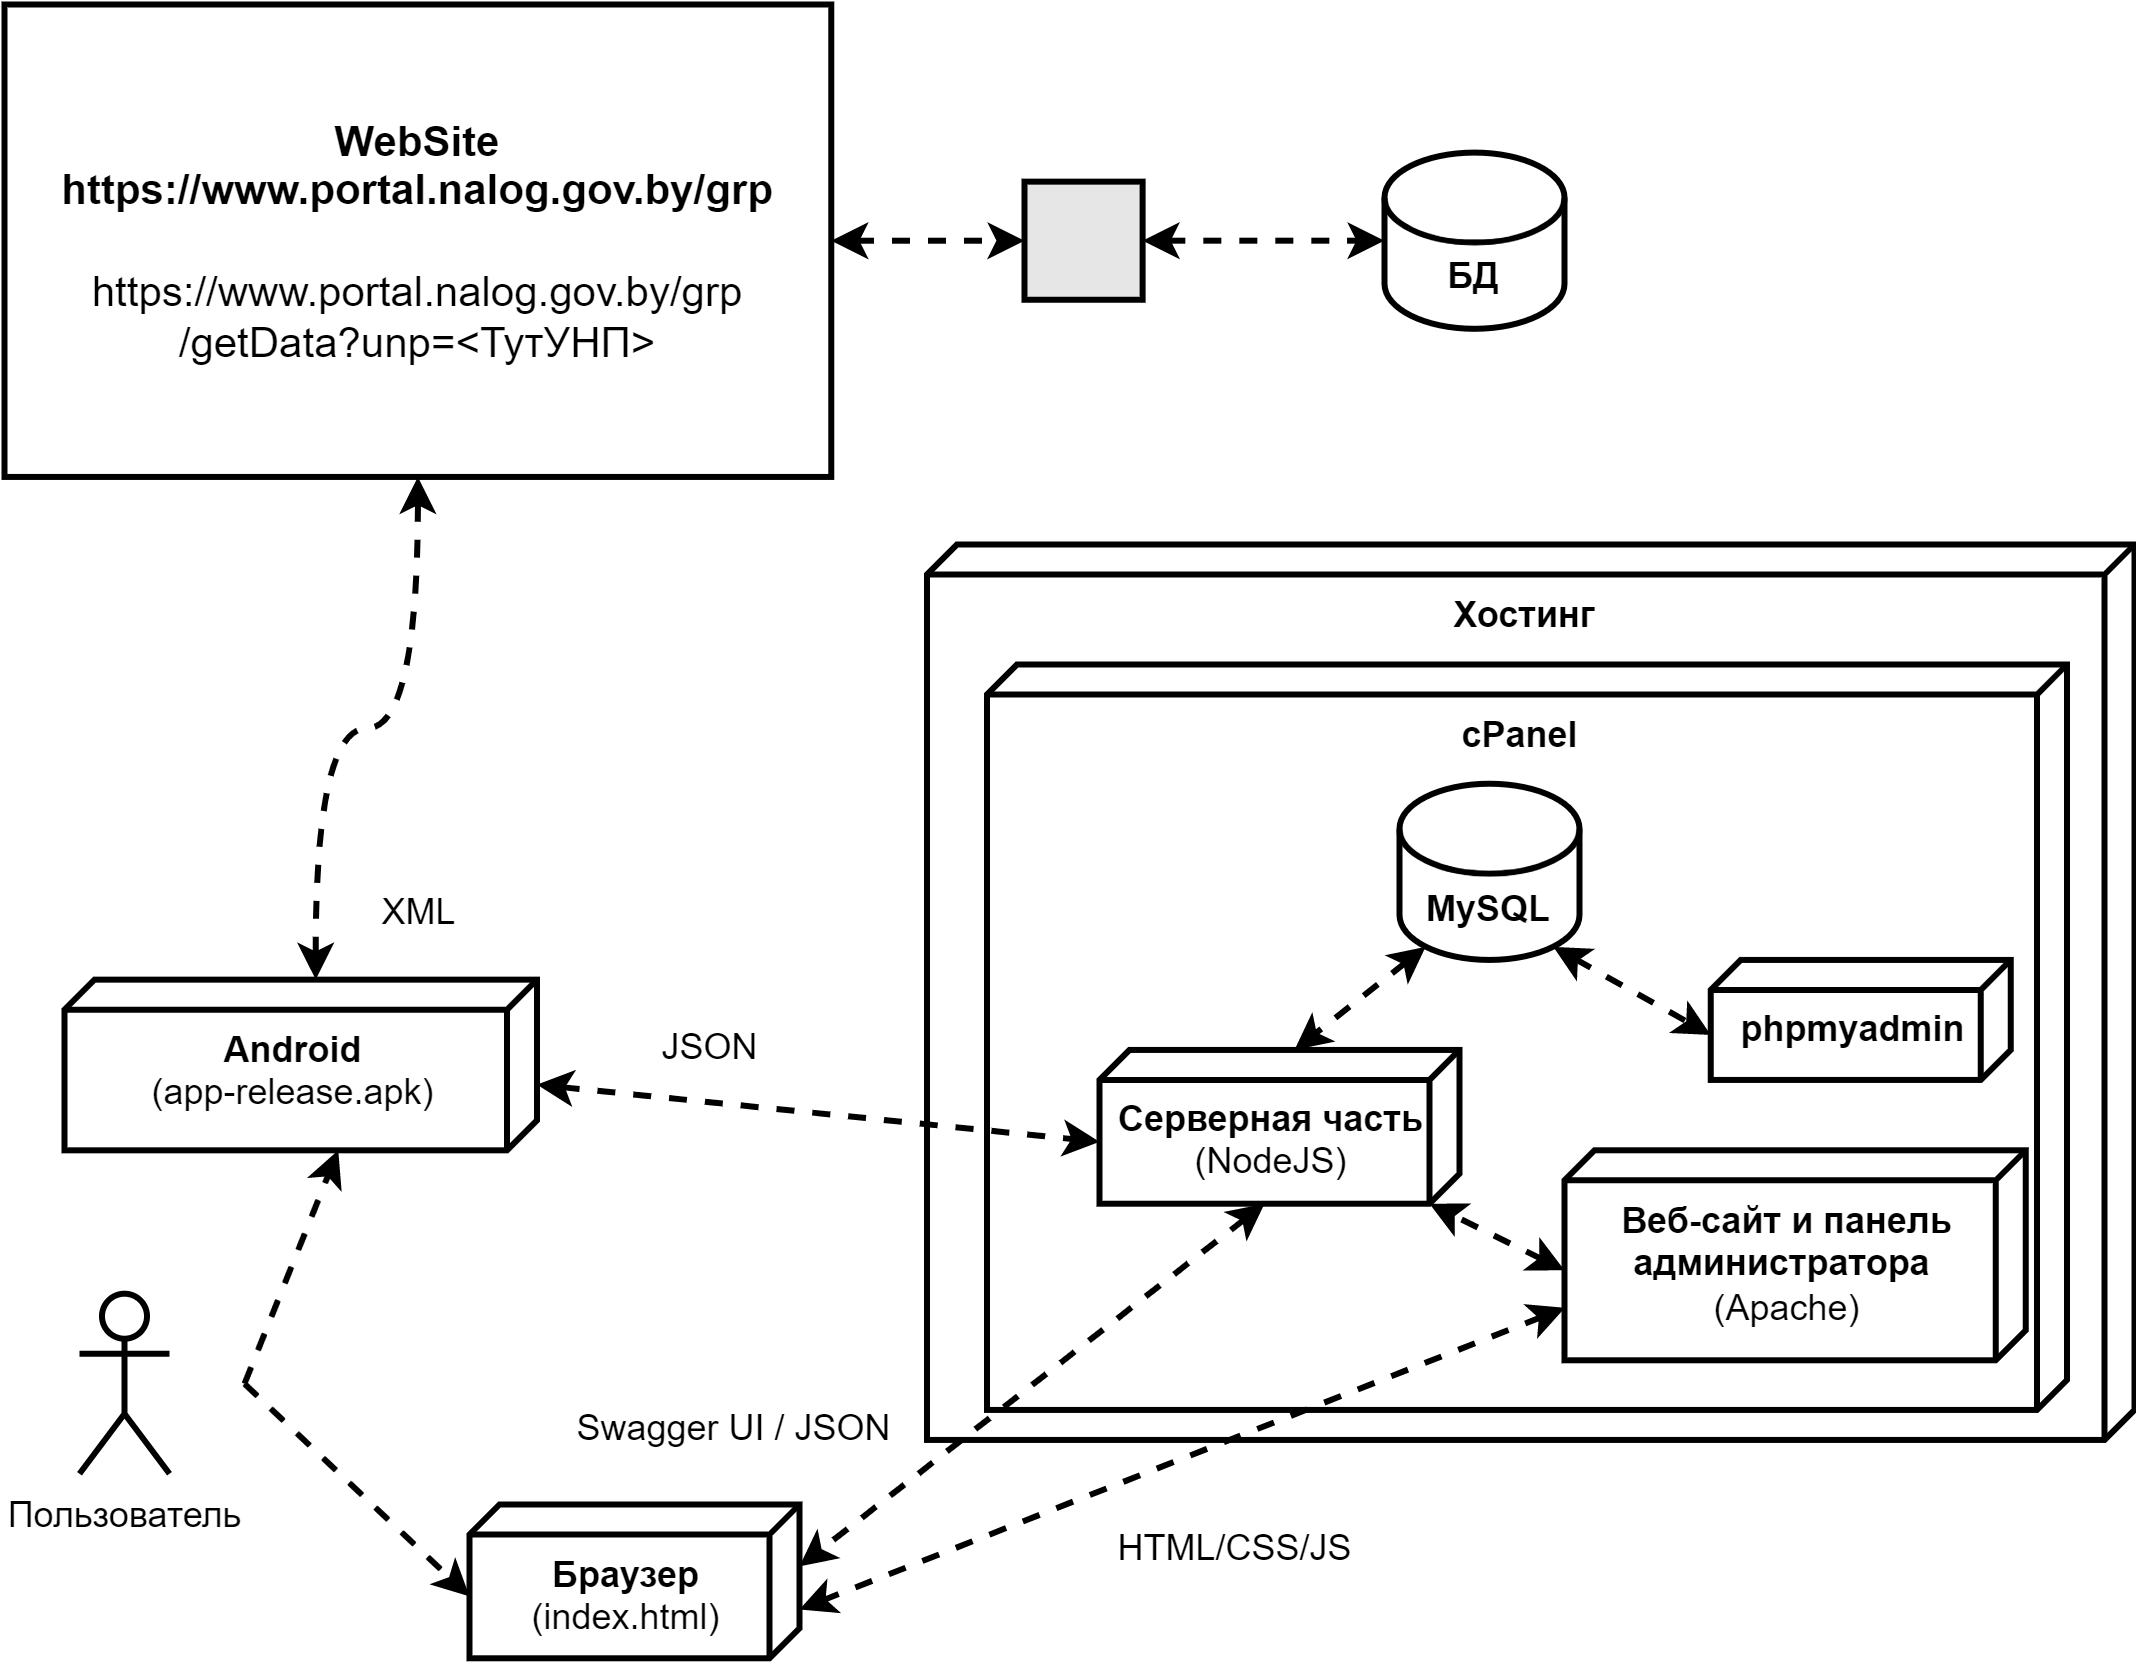
\includegraphics[width=18cm]
    {images/UML/UML_deployment_diagram_prod.png}

    \caption{Диаграмма развертывания приложения}

    \label{fig:UML_deployment_diagram_prod}
\end{figure}
